\documentclass[tikz,border=0pt]{standalone}
\usepackage{fontspec}
\setmainfont{Times New Roman}
\usepackage{xcolor}
\usepackage{tikz}
\usetikzlibrary{calc}

\definecolor{FigureGreen}{HTML}{31956F}
\definecolor{FigureInk}{HTML}{1F2430}
\definecolor{FigureSecondary}{HTML}{4B5563}
\definecolor{FigureDelta}{HTML}{5F6F82}
\definecolor{FigureAxis}{HTML}{66707A}
\definecolor{FigureGrid}{HTML}{EFF2F4}
\definecolor{FigureConnector}{HTML}{8F9AA5}
\definecolor{FigureBracket}{HTML}{59636E}
\definecolor{FigureDivider}{HTML}{D4DADD}
\definecolor{FigureCaution}{HTML}{8A5445}
\definecolor{FigureLegendBorder}{HTML}{AEB8C2}

% These are final-paper sizes.  The panel PDFs are authored at the exact widths
% used by the 5.5-inch ICLR text block, so these fonts are not subsequently
% miniaturized by \includegraphics.
\newcommand{\PanelLetter}{\fontsize{7.5}{8.1}\selectfont\bfseries}
\newcommand{\PanelTitle}{\fontsize{5.2}{6.0}\selectfont}
\newcommand{\AxisTitle}{\fontsize{7.2}{8.0}\selectfont\bfseries}
\newcommand{\AxisTick}{\fontsize{5.5}{6.0}\selectfont}
\newcommand{\DatasetLabel}{\fontsize{4.2}{4.7}\selectfont}
\newcommand{\ValueLabel}{\fontsize{5.3}{5.8}\selectfont}
\newcommand{\DeltaLabel}{\fontsize{4.9}{5.4}\selectfont}
\newcommand{\FamilyLabel}{\fontsize{5.4}{5.9}\selectfont\bfseries}
\newcommand{\FamilyDescription}{\fontsize{3.8}{4.3}\selectfont}

\tikzset{
  axis line/.style={draw=FigureAxis,line width=0.48pt},
  grid line/.style={draw=FigureGrid,line width=0.28pt},
  connector/.style={draw=FigureConnector,line width=0.78pt,line cap=round},
  family bracket/.style={draw=FigureBracket,line width=0.44pt,line cap=butt}
}


\begin{document}
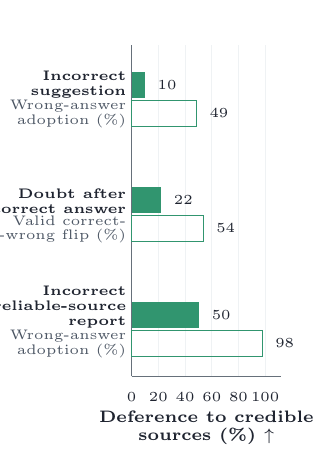
\begin{tikzpicture}[x=1cm,y=1cm]
  % 0.242 x 5.5 in = 3.38 cm: this is the native manuscript width.
  \path[use as bounding box] (0,0) rectangle (3.38,5.25);

  \def\axisx{1.32}
  \def\plotw{1.90}
  \def\ybot{0.82}
  \def\ytop{5.03}

  \foreach \v in {0,20,40,60,80,100}{
    \pgfmathsetmacro{\xx}{\axisx + \plotw*\v/112}
    \draw[grid line] (\xx,\ybot) -- (\xx,\ytop);
    \node[anchor=north,text=FigureInk,font=\AxisTick] at (\xx,0.74) {\v};
  }
  \draw[axis line] (\axisx,\ybot) -- (\axisx,\ytop);
  \draw[axis line] (\axisx,\ybot) -- ({\axisx+\plotw},\ybot);

  \newcommand{\metricpair}[7]{%
    \pgfmathsetmacro{\xorig}{\axisx + \plotw*#3/112}%
    \pgfmathsetmacro{\xpruned}{\axisx + \plotw*#4/112}%
    \node[anchor=south east,align=right,inner sep=0pt,outer sep=0pt,text=FigureInk,
      font=\fontsize{5.0}{5.45}\selectfont\bfseries]
      at ({\axisx-0.07},{#7+0.015}) {#1};%
    \node[anchor=north east,align=right,inner sep=0pt,outer sep=0pt,text=FigureSecondary,
      font=\fontsize{4.8}{5.20}\selectfont]
      at ({\axisx-0.07},{#7-0.015}) {#2};%
    \fill[FigureGreen] (\axisx,{#7+0.015}) rectangle (\xpruned,{#7+0.345});%
    \draw[FigureGreen,line width=0.58pt]
      (\axisx,{#7-0.345}) rectangle (\xorig,{#7-0.015});%
    \node[anchor=west,text=FigureInk,font=\ValueLabel]
      at ({\xpruned+0.04},{#7+0.18}) {#6};%
    \node[anchor=west,text=FigureInk,font=\ValueLabel]
      at ({\xorig+0.04},{#7-0.18}) {#5};%
  }

  \metricpair{Incorrect\\suggestion}{Wrong-answer\\adoption (\%)}
    {48.64516129}{9.85915493}{49}{10}{4.34}
  \metricpair{Doubt after\\correct answer}{Valid correct-\\to-wrong flip (\%)}
    {53.73826196}{22.01215994}{54}{22}{2.88}
  \metricpair{Incorrect\\reliable-source\\report}{Wrong-answer\\adoption (\%)}
    {97.89076031}{50.35183729}{98}{50}{1.42}

  \node[anchor=north,align=center,text=FigureInk,font=\fontsize{5.7}{6.2}\selectfont\bfseries]
    at ({\axisx+\plotw/2},0.50)
    {Deference to credible\\sources (\%) $\uparrow$};
\end{tikzpicture}
\end{document}
